\section{Evaluations}
\label{evaluation}

We evaluate our algorithms in distributed settings with 20 Amazon EC2 m1.xlarge machines. Each machine has 4 vCPUs and 15 GiB memory. We use Powergraph \cite{180251} as the platform to implement the distributed version. We also implemented a centralized version with Snap \cite{snapnets}. All algorithms are implemented in C++.

\subsection{Datasets}

\begin{table}
    \centering
    \begin{tabular}{|c|c|c|c|} \hline
        Dataset & Type & $|V_{wcc}|$ & $|E_{wcc}|$ \\ \hline
        Google & Web & 856K & 4.3M \\ \hline
				Wiki-talk & Communication & 2.4M & 4.7M \\ \hline
        Skitter & Internet & 1.7M & 11.1M \\ \hline
        Mouse-gene & Biological & 43K & 14.5M \\ \hline
				%Patent & Collaboration & 3.8M & 16.5M \\ \hline
				Baidu & Web & 2.1M & 17.0M \\ \hline
        Facebook & Social & 3.1M & 23.7M \\ \hline
        Livejournal & Social & 4.8M & 43.4M \\ \hline
        Hollywood & Collaboration & 1.1M & 56.3M \\ \hline
        Friendster & Social & 65M & 1.8B \\ \hline
    \end{tabular}
    \caption{Datasets}
    \label{table:datasets}
\end{table}

We evaluate our algorithm on 9 graphs from different disciplines as shown in table \ref{table:datasets} in ascending order on the number of edges. All graphs are complex networks that have power-law degree distribution and relatively small diameter. All datasets have at least millions of edges, the largest one has more than one billion edges. To simplify our experiments, we treat each graph as undirected, un-weighted graphs. We only use the largest weakly connected component of each graph that consist of more than $90\%$ of vertices for all graphs. All datasets are collected from \cite{snapnets} and \cite{nr}.

\subsection{Approximation Accuracy}
\label{eval_accuracy}

In order to evaluate the performance of decentralized search and various optimizations, we compare the distance of estimated path and true distance of vertex pairs. To control the number of exact pairs of shortest path distance we need to find using BFS, we randomly choose 1,000 vertices of each graph as source vertices. For each source vertex, we randomly choose 100 vertices as target vertices. All the results in Fig. \ref{fig:accuracy_dec} and Fig. \ref{fig:accuracy_index} are averaged with 100,000 queries.

\begin{figure*}[t]
    \centering
    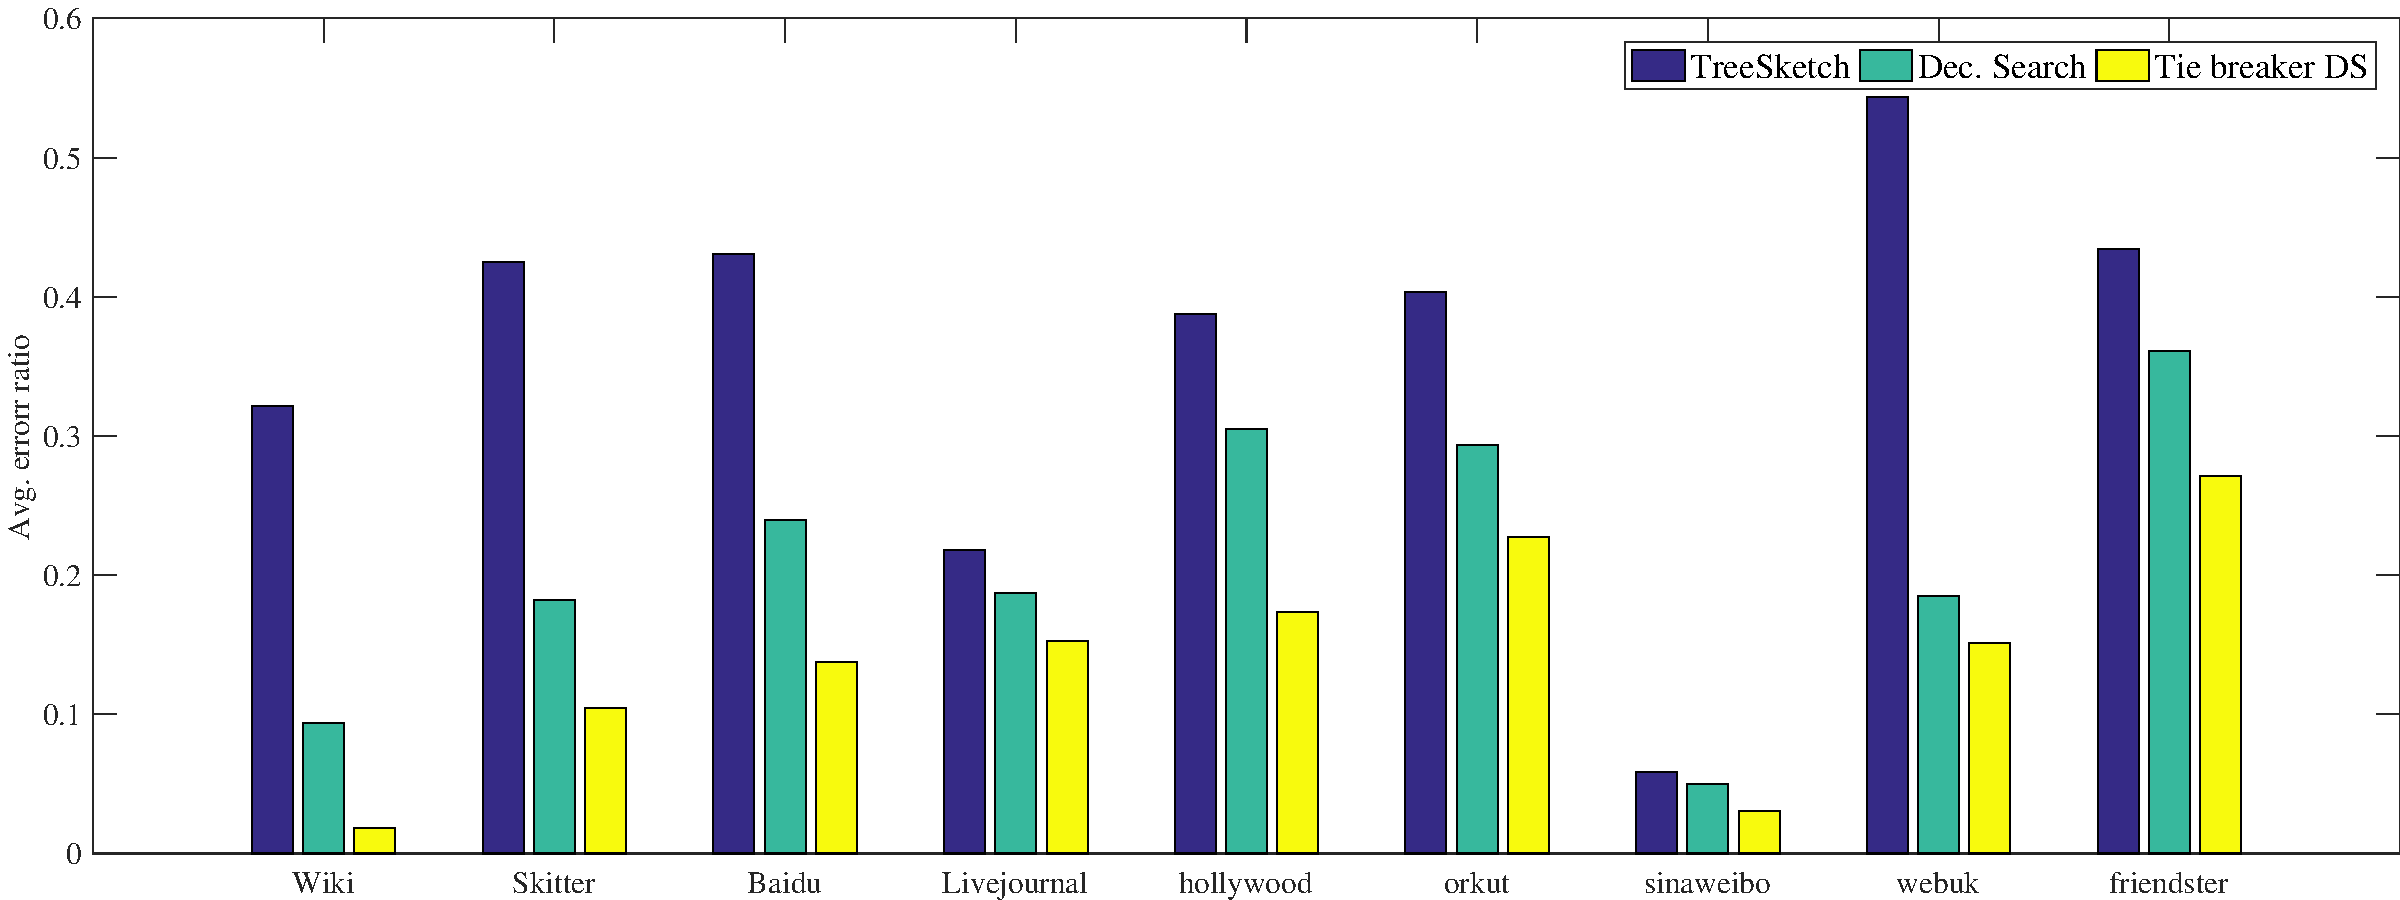
\includegraphics[width=\linewidth]{../figures/accuracy_dec.pdf}
    \caption{The accuracy of the approximated distance of decentralized search and various optimizations compared to LCA distance.}
    \label{fig:accuracy_dec}
\end{figure*}

We first compare the accuracy of decentralized search and LCA distance. For the decentralized search, we also compare accuracy of various optimizations including bidirectional search, distributed tie breaking strategy and greedy index construction to achieve different level of accuracies. The accuracy gain is shown in Fig. \ref{fig:accuracy_dec}. All experiments are carried on with $2$ landmarks except last one using $20$ landmarks (note that we cannot construct a $20$ landmark index for graph friendster due to the hardware limitations). From the figure, we can see that decentralized search achieves better accuracy for all graphs, and the performance gain varies from $8\%$ to $64\%$. Various optimizations also have great impact on the accuracy. When all three optimizations have been used, the accuracy are even better than LCA distance computed from $20$ landmarks for $7$ out of $8$ graphs (not including the graph friendster).

%\begin{figure}[t]
    %\centering
    %\includegraphics[width=\linewidth]{../figures/accuracy_compare.pdf}
    %\caption{The accuracy of estimated distance of decentralized search compared to code comparison when number of landmarks increase.}
    %\label{fig:accuracy_compare}
%\end{figure}

%we show that as the number of landmarks increase, the decentralized search still out performs comparison based algorithms a lot, that is, even when we have a relatively large landmark set which require more time and storage overhead to construct, it's still had to achieve same level of accuracy by using decentralized search. For example, decentralized search with 2 landmarks outperform comparison based algorithm with 20 landmarks. With 20 landmarks, decentralized search can find exact shortest path for most of pairs. \comment{put some number here when the figure is final.}

\begin{figure}[t]
    \centering
    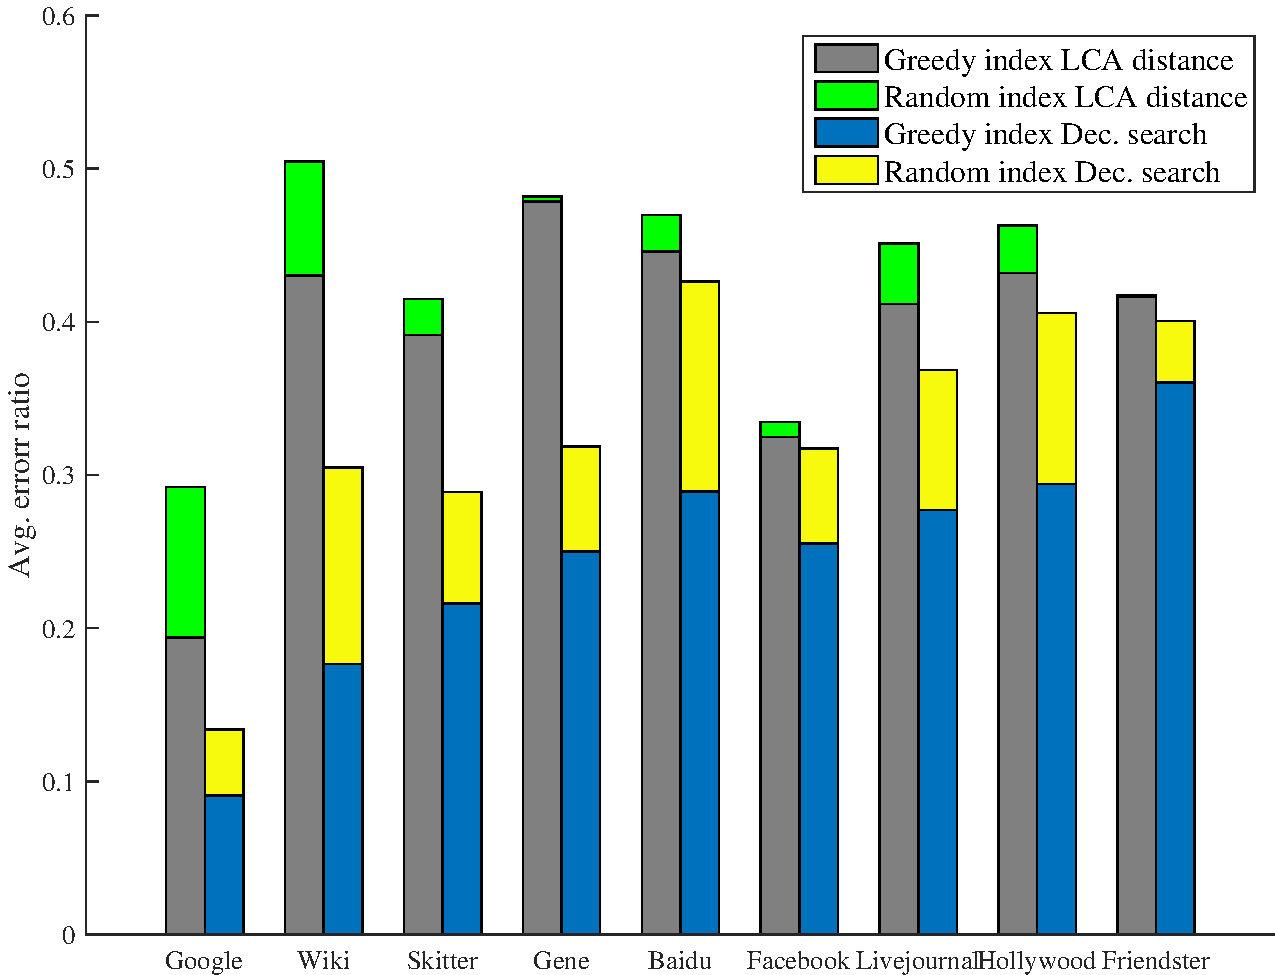
\includegraphics[width=\linewidth]{../figures/accuracy_index.pdf}
    \caption{Impact of index quality on the accuracy of both decentralized search and label comparison.}
    \label{fig:accuracy_index}
\end{figure}

We then evaluate our heuristic index construction algorithm compared to the random index construction algorithm. We compared the results of decentralized search and LCA distance on both kinds of indexes. Fig. \ref{fig:accuracy_index} shows the performance gain for a single landmark. As we can see that indexes created by greedy heuristic have a much smaller average error rate for both decentralized search and LCA computation. Due to that decentralized search examine more pairs of vertices than LCA computation, it has a better performance gain on $8$ out of $9$ graphs compared to LCA computation.

\subsection{Overhead}
\label{eval_overhead}

We study the preprocessing and online search overhead of decentralized search in this section. First we compare the preprocessing overheads of greedy index construction with random index construction. Then for online search overheads, to show the impact of increased search space, we compare the average search time with various optimizations enabled. 

\begin{figure}[t]
    \centering
    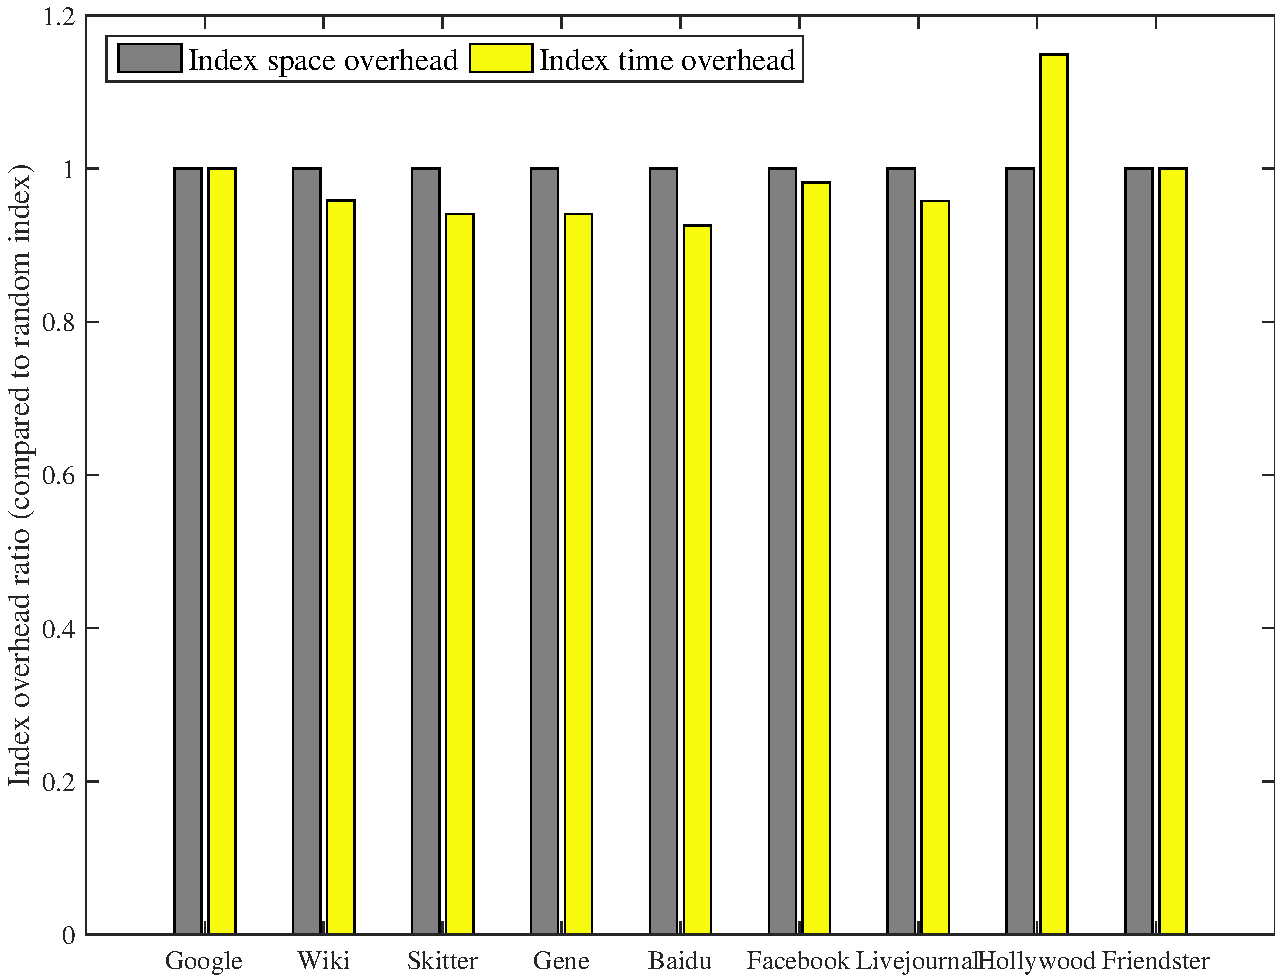
\includegraphics[width=\linewidth]{../figures/overhead_index.pdf}
    \caption{The time and space overhead for preprocessing for a single landmark by heuristic and random index construction}
    \label{fig:overhead_index}
\end{figure}

Since whenever the shortest path to the landmark are indexed, they have the same path length, so the space overhead are exactly the same. This can be seen in Fig. \ref{fig:overhead_index} that greedy index construction algorithm brings no extra space overhead. Greedy index construction has limited time overhead too. Since the only additional operation of the algorithm is to calculate the sum of degree along each path, which takes constant time in our implementation. Actually, the difference of time overhead mainly comes from the number of times a label has been updated according to path degree or randomly. We can see in Fig. \ref{fig:overhead_index} that both preprocessing algorithms have similar time overhead.

\begin{figure}[t]
    \centering
    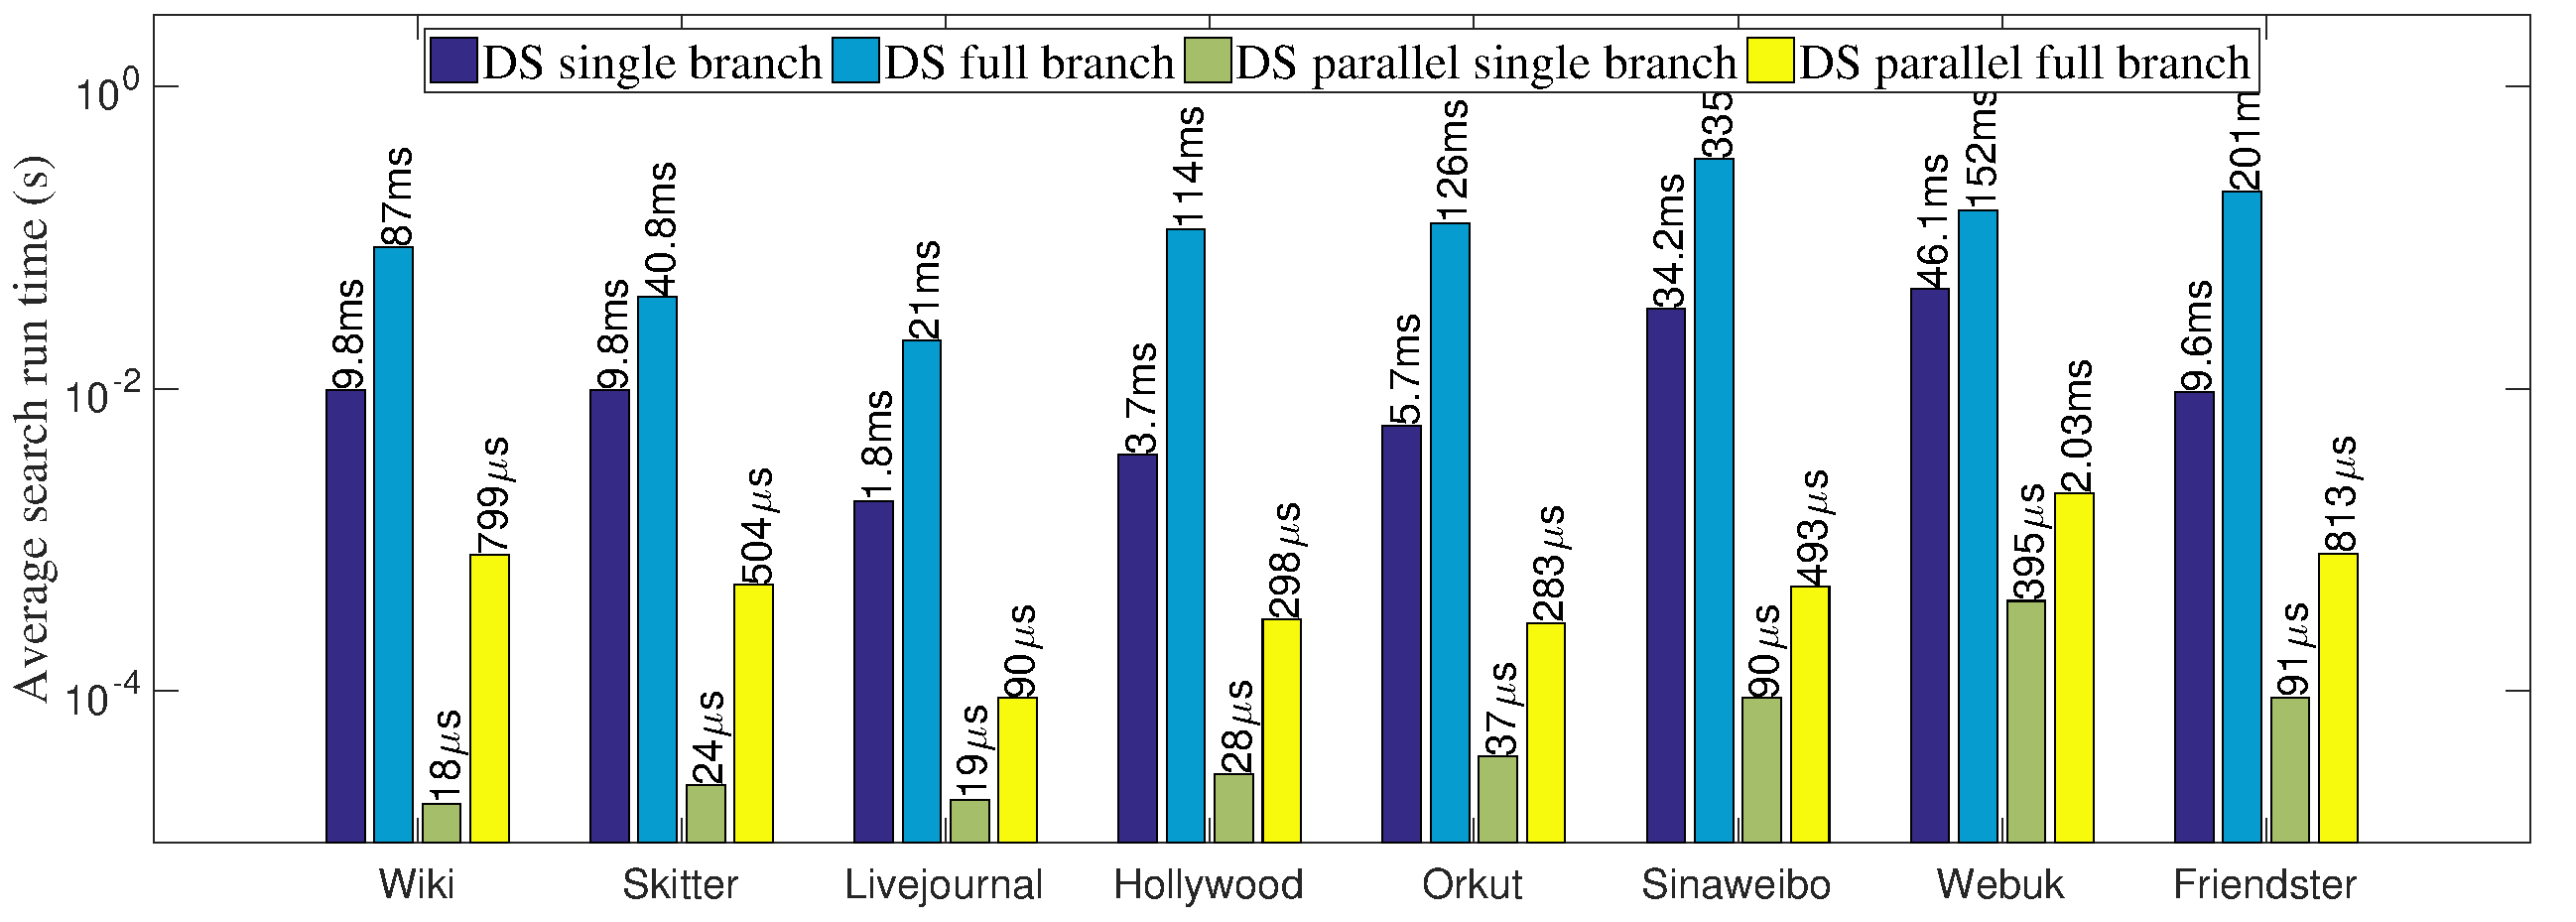
\includegraphics[width=\linewidth]{../figures/overhead_search.pdf}
    \caption{The average search time of decentralized search with various optimizations.}
    \label{fig:overhead_search}
\end{figure}

Fig. \ref{fig:overhead_search} shows the online search overhead in log scale with different optimizations. Note that results for bidirectional search and tie breaking are both with early termination on. We can see that early termination greatly reduces the search overhead from $71.6\%$ to $99.7\%$ by reducing the number of vertices being examined. The time overhead of bidirectional search shown in Fig. \ref{fig:overhead_search} is $2.42$ to $4.38$ times more than one direction search due to it has to found two paths instead of one path. The situation is a little complicated for tie breaking, since it is more related to the structure of each graph. For most graphs, the time overhead is $2.74$ to $16.71$ times more than one direction search. The worst case is $109.53$ for graph mouse-gene which is the densest graph in our datasets, where too many candidates with same LCA distance exist at each step.

\subsection{Scalability}
\label{eval_scalability}

Since our algorithm is designed for large-scale networks, scalability is another major concern of our algorithm. Due to that we implement the algorithm in a distributed setting and execute queries in a parallel way, we study how our algorithm performs when number of machines and queries changes. Moreover, as the size of graph is expected to further increasing in the future, we also studies the impact of the size of the graph to our algorithm.

\begin{figure}[t]
    \centering
    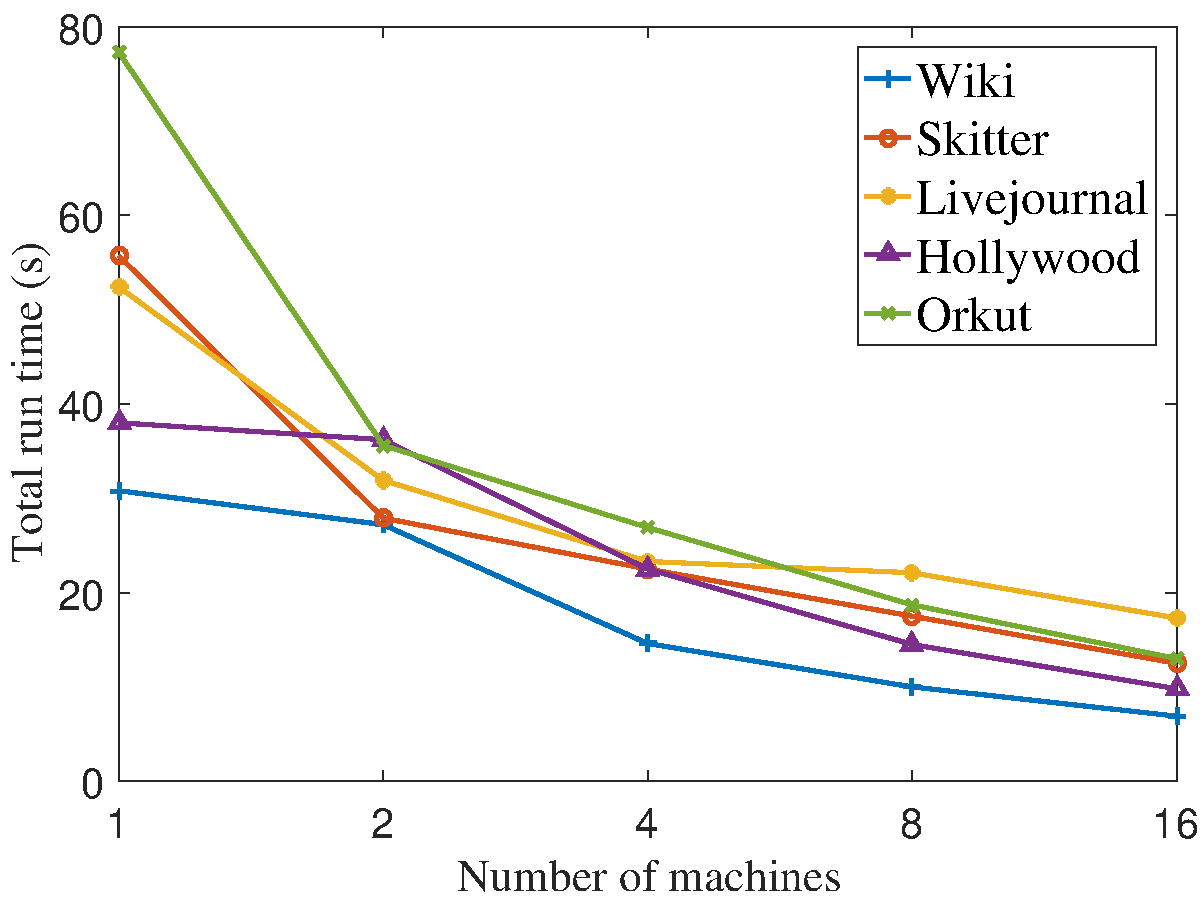
\includegraphics[width=\linewidth]{../figures/scale_machine.pdf}
    \caption{The average search time as the number of machines increase}
    \label{fig:scale_machine}
\end{figure}

We first evaluate the search time when number of machines increasing. Results shown in Fig. \ref{fig:scale_machine} are averaged of 1,000,000 queries. We can see the trend is that the average run-time decreases as the number of machines increase. The average search time decreases fast when small number of machines are deployed and slow down when large number of machines are used. However there are some spikes in the curve, which might be caused by the hot-spot problem we mentioned before.

\begin{figure}[t]
    \centering
    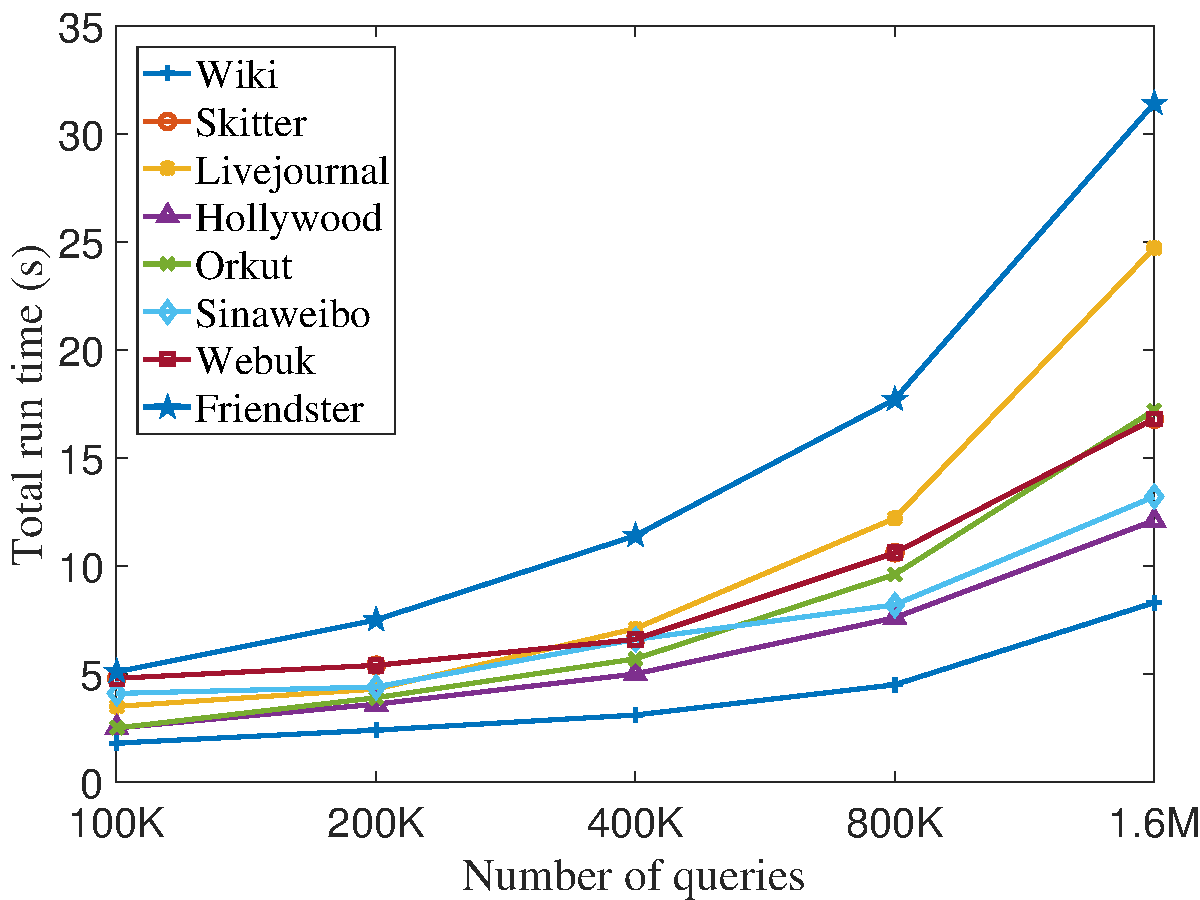
\includegraphics[width=\linewidth]{../figures/scale_query.pdf}
    \caption{The average search time as the number of queries increase}
    \label{fig:scale_query}
\end{figure}

%\begin{table*} [ht]
    %\centering
    %\begin{tabular}{cccccccccc} \hline
				%&Google&Wiki&Skitter&Gene&Baidu&Facebook&Livejournal&Hollywood&Friendster \\ \hline
				%Tie(centralized)&85.0&96.9&33.0&41.1&143.29&31.1&36.6&12.7&N/A \\ \hline
				%Tie(distributed)&3.6&40.3&12.4&6.73&43.8&2.8&3.9&3.2&2.1 \\ \hline
    %\end{tabular}
    %\caption{Number of paths returned by decentralized search with different tie breaking strategies}
    %\label{table:NOP}
%\end{table*}

We then examine average search time as number of queries running in parallel increases. All experiments are carried on 20 machines in this part. We can see in Fig. \ref{fig:scale_query} that the average search time quickly goes down when the number of queries is small. The reason is that there are some fixed overheads to start and stop the engine for a batch of queries. When the number of queries increases, the average overhead for each query will decrease. But when the number of queries becomes larger, the average search time begins to go up.  Because too many searches will reach the memory and communication limits, that slow down the search speed.

\begin{figure}[t]
    \centering
    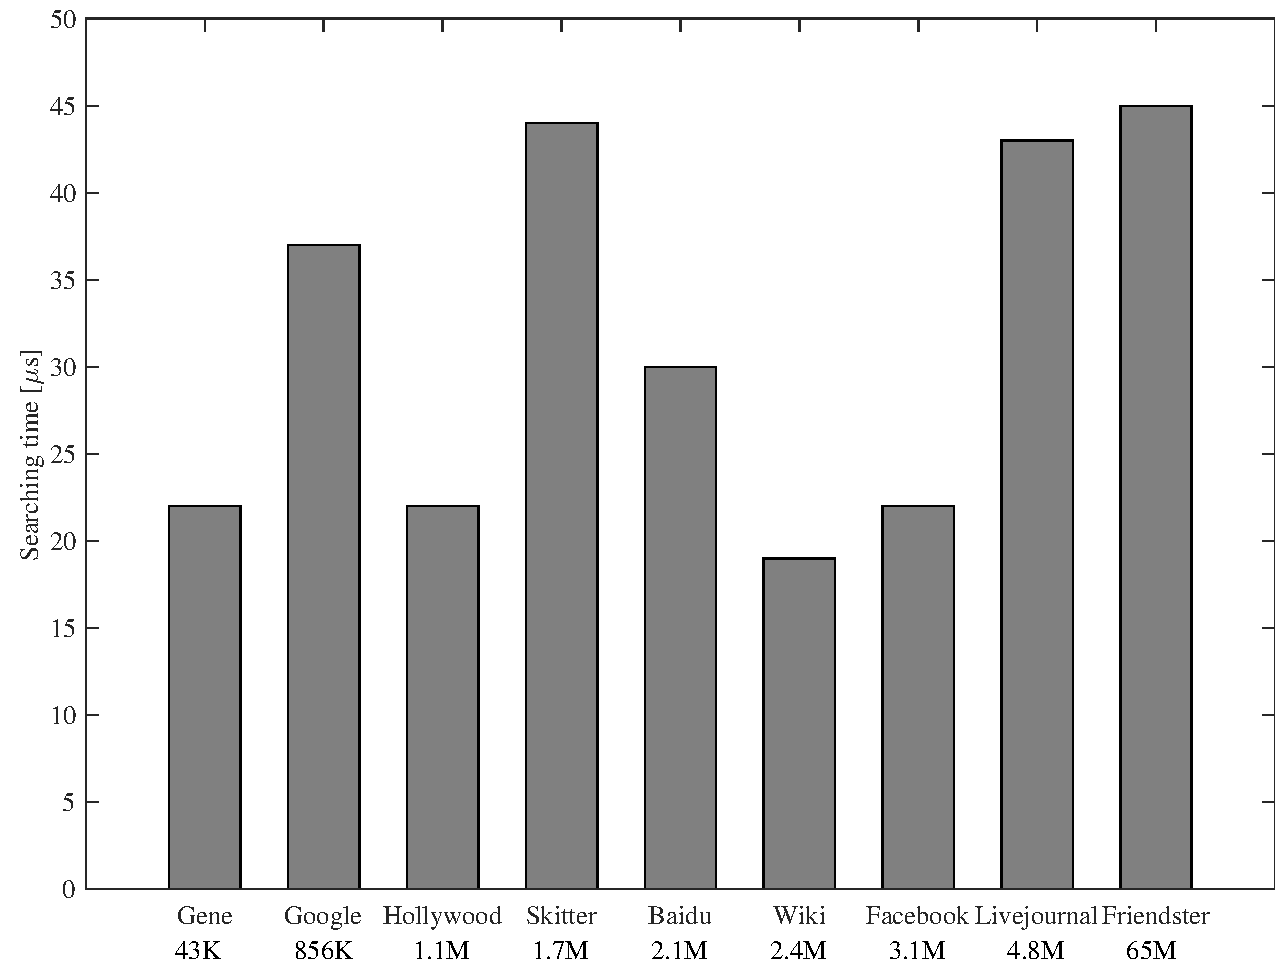
\includegraphics[width=\linewidth]{../figures/scale_graph.pdf}
    \caption{The average search time for different size of graphs}
    \label{fig:scale_graph}
\end{figure}

In the last experiment, we evaluate the search time as the size of graph increases. Unlike BFS which needs to traverse neighbors of $O(n)$ vertices, decentralized search only needs to exam neighbors of $O(log(n))$ vertices for complex networks due to the small world property. We can clearly see in Fig. \ref{fig:scale_graph} that as the number of vertices increases, average search time of decentralized search does not follow the same trend. The graph friendster which have sixty-five millions vertices have average search time only $2.05$ times more than graph mouse-gene which only have forty-three thousand vertices.

%\subsection{Path Diversity}
%\label{eval_diversity}
%
%The number of paths returned by decentralized search are heavily relied on tie breaking strategies. The more vertices the search selects when tie happens, the more paths it will return. Fig. \ref{table:NOP} shows average number paths returned by two tie breaking strategies. The first one is used in our centralized implementation, where all neighbors with same LCA distance are selected. The second one is used in our distributed implementation, where only one neighbor is marked as "main" candidate. We can see that the tie strategy we used in centralized settings can return far more paths than the strategy we used in distributed settings because of the larger search space. We don't have centralized version for graph friendster because it is too large to fit in one machine.

%\subsection{for dynamic graphs}
%The robustness of decentralized search against graph changes mainly comes from the property that decentralized search can explore multiple paths at the same time. Usually for an arbitrary source and target pair, there are not only one unique paths among them but several paths with various length. Since decentralized search is not exact algorithm, so it may not find the shortest one most of the time. But it can find several paths with same approximation length. So even for dynamic graphs where edges appear and disappear as time changes, decentralized search is still able to find valid paths.

%\subsection{error distribution}
%
%\begin{figure}[t]
    %\centering
    %\includegraphics[width=\linewidth]{../figures/empty.pdf}
    %\caption{Distribution of errors of different length}
    %\label{fig:distribution}
%\end{figure}
%
%\comment{we want to show that the algorithm performs equally well for various path length}
%In the last, we study the error distribution according to the length of exact shortest path.
